\chapter{Intrusion Detection and Prevention Systems}

Intrusion Detection (and Prevention) Systems (from now on, IDS and/or IPS) are particular HW/SW systems developed to detect security threats in a computer system.\newline
Historically, they were developed using signature-based techniques, that is: you define an attack pattern and, if ot recognize that exact pattern in the system's activity, it raises an alarm.\newline\newline
Since Machine Learning is one of the increasing trends, gaining more and more popularity, we began to think if, instead of defining the "attack pattern" (or signature) for a particular malicious activity, we could define the "good behaviour" for users and program to detect malicious behaviour and here is where anomaly-based IDS comes in.

\subsection{Machine Learning and IDS combined}

Let's get more into the interesting things now. The first question is: How do I define the "normal" behaviour for users and programs? We need to have a dataset representing these behaviours. We have two alternatives:

\begin{itemize}
	\item Stateful Protocol Analysis
		\begin{itemize}
			\item[$\rightarrow$] We buy these datasets from authorized vendors. These data are usually very accurate and very little work is needed on them. The bad thing? The price is usually very high
		\end{itemize}
	\item Collect data by ourselves
		\begin{itemize}
			\item[$\rightarrow$] This approach is usually less expensive but require much more work on the data (such as \emph{feature selection}). For the purpose of this course we will have a better look at this approach, since it allows us to use some more statistical techniques
		\end{itemize}
\end{itemize}

Data are collected by the IDS using a \emph{sensor} (an HW or SW module). These data are sent to an \emph{analyzer} that compares them with the ones collected in the training phase, in order to detect intrusions. However, the very big problem with these kind of systems is that we want a very small number of \emph{false positives} and \emph{false negatives}, otherwise the whole system is useless!\newline\newline
This is the main reason why we will put some emphasis to \emph{feature selection} and \emph{feature classification}\newline\newline

Roughly, the process used to build this kind of system is depicted in Figure 1:
	\begin{itemize}
		\item[1)] First of all we need a \emph{Train Set}, to tell the system what are the accepted behaviours
		\item[2)] Now that we have only the relevant components in our train set, we can classify data. Empirically, it has been observed that \emph{Decision Tree} provides the higher accuracy for anomaly detection
		\item[3)] At this point we are able to test our system with a \emph{Test Set}, to check the accuracy of our model of correctly detecting intrusions
	\end{itemize}
	
	\begin{figure}[h!]
		\centering
		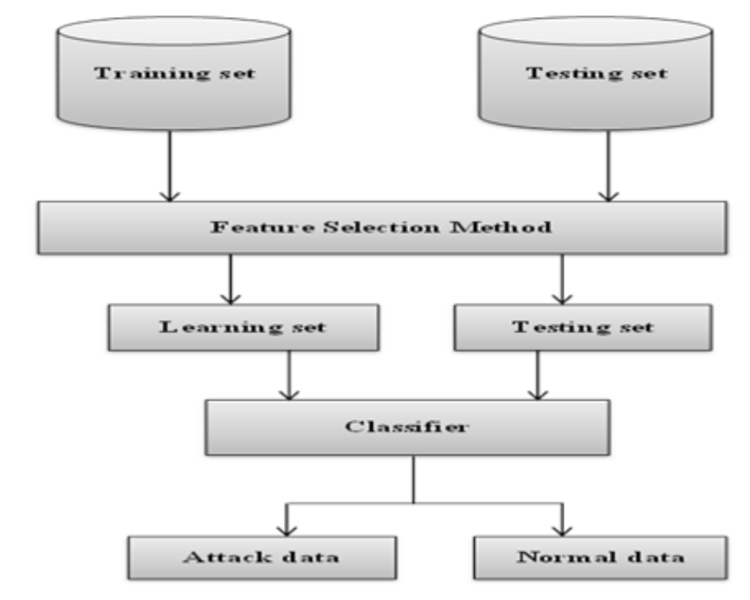
\includegraphics[width=\textwidth,height=8.5cm]{img/IDSPhases.png}
	\end{figure}